% um seins alleine (ohne labels des anderen) zuarbeiten ein % davor weg 
% standart einstellung ist alleine arbeiten 
%!TeX root = Vorlage_nur_inhalt2.tex
% um das gesammte dokuemnt zu erstellen oder um die labels des anderen zu nutzen einmalig ein % wegmachen und nach dem man fertig ist wieder ein % zeichen davor und bei der zeile darüber ein % weg sodass %!... steht
%% !TeX root = ../Inhalt_1+2/Vorlage.tex
%a%!TEX projectfile = ../header/seiten_einstellungen.tex
%a%!TEX projectfile = header.tex
%a%!TEX projectfile = ../Inhalt2/inhalt2.tex.tex
%!TEX projectfile = ../Inhalt1/inhalt1.tex.tex

\resetlaborsectioncounter
\laborsubsection{D}{Funktion f(x) in Latex}
\begin{figure}[H]
	\centering
	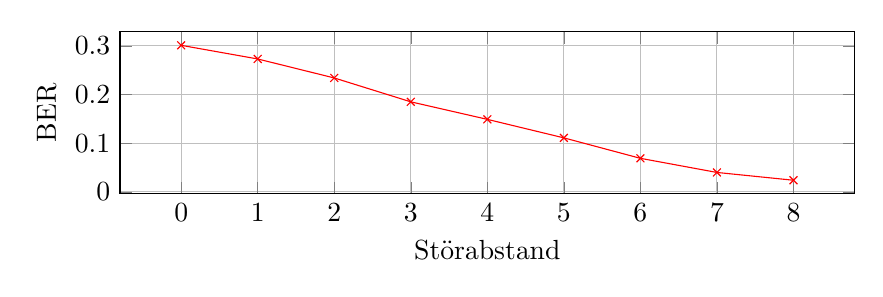
\begin{tikzpicture}
		\begin{axis}[
			xlabel=Störabstand,
			ylabel=BER,
			grid=major,
			width=0.9\textwidth,
			height=0.3\textwidth]
			\addplot[color=red,mark=x] coordinates {
				(0,0.301)
				(1,0.273)
				(2,0.234)
				(3,0.185)
				(4,0.149)
				(5,0.111)
				(6,0.069)
				(7,0.04)
				(8,0.024)
			};
		\end{axis}
	\end{tikzpicture}
	\caption{Diagramm aus Koordinaten}
	\label{fig:2_2_diagramm}
\end{figure}


\newpage
\section{Programmiersprachen sämtlicher Art}
\laborsubsection{D}{Ja auch MATLAB}\label{code:matlab}
\begin{lstlisting}[language=matlab]
	syms x;
	c0 = 0;
	c1 = 1;
	c2 = 0.1;
	c3 = -0.05;
	X = 2; % X = 1;
	Y1dach = c1*X + (3/4)*c3*X^3;
	Y2dach = (1/2)*c2*X^2;
	Y3dach = (1/4)*c3*X^3;
	Y1eff = (1/sqrt(2)) * Y1dach;
	Y2eff = (1/sqrt(2)) * Y2dach;
	Y3eff = (1/sqrt(2)) * Y3dach;
	Ygeseff = sqrt(Y1eff^2 + Y2eff^2 + Y3eff^2);
	
	k2 = Y2eff/Ygeseff
	k3 = Y3eff/Ygeseff
	kges = sqrt(k2^2 + k3^2)
	
\end{lstlisting}








\newpage
\section*{Geräteliste}
\begin{table} [H]
	\label{tab:geraeteliste}
	\begin{tabular}{|l|l|}
		\hline
		\textbf{Gerät }            & \textbf{Nummer }            \\ \hline
		Multimeter Keysight U1241C & AMES\_13, AMES\_14,AMES\_15 \\ \hline
		Stelltrafo                 & 27-15                       \\ \hline
		Stelltrafo                 & 29-24                       \\ \hline
		Ringkerntrafo              & 97-24                       \\ \hline
		Digitalmultimeter          & 40-24                       \\ \hline
	\end{tabular}
\end{table}
